\documentclass[12pt, a4paper]{article}
\usepackage{xcolor}
\usepackage[top=2cm, bottom=2cm, left=2.0cm, right=2.0cm]{geometry}
\geometry{a4paper}
\usepackage{tikz}
\usetikzlibrary{trees, positioning, shapes, arrows.meta, shapes.geometric}
\usepackage{forest}
\usepackage{amsmath}
\usepackage{algorithm}
\usepackage{algpseudocode}

\begin{document}

\title{Monte Carlo Tree Search (MCTS)\\ 
A Comprehensive Visual Guide}
\author{Christophe Louargant}
\date{\today}
\maketitle

\begin{abstract}
This document provides a comprehensive visualization of
Monte Carlo Tree Search algorithms applied to zero-sum 
two-player games.
Through step-by-step tree diagrams and detailed explanations,
we demonstrate how these methods work for two-player games
like HEX. We explore the algorithm's components, including
the minimax perspective, random playouts, and UCB1 selection
strategy.
\end{abstract}

\section*{Introduction to Monte Carlo Tree Search}

Monte Carlo Tree Search (MCTS) is a heuristic search
algorithm that combines the precision of tree search
with the generality of random sampling. Unlike traditional
minimax algorithms that require evaluation functions,
MCTS uses random playouts to estimate the value of positions.\\
%
MCTS combines three powerful ideas:

\begin{center}
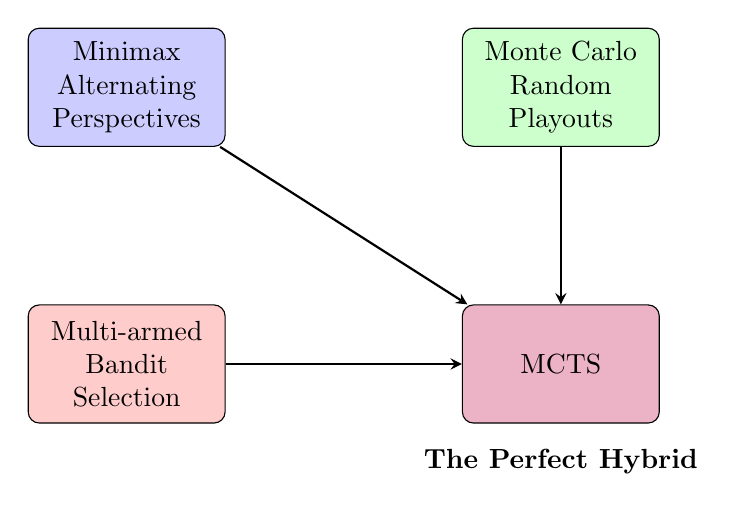
\begin{tikzpicture}[
    concept/.style={rectangle, draw, rounded corners, align=center, minimum width=2.5cm, minimum height=1.5cm},
    arrow/.style={->, >=stealth, thick}
]

\node[concept, fill=blue!20] (minimax) {Minimax\\Alternating\\Perspectives};
\node[concept, fill=green!20, right=3cm of minimax] (montecarlo) {Monte Carlo\\Random\\Playouts};
\node[concept, fill=red!20, below=2cm of minimax] (bandit) {Multi-armed\\Bandit\\Selection};
\node[concept, fill=purple!30, below=2cm of montecarlo] (hybrid) 
{MCTS};

\draw[arrow] (minimax) -- (hybrid);
\draw[arrow] (montecarlo) -- (hybrid);
\draw[arrow] (bandit) -- (hybrid);

\node[below=0.2cm of hybrid] {\textbf{The Perfect Hybrid}};
\end{tikzpicture}
\end{center}

\subsection*{The Magic Formula}

\[
\text{MCTS} = \text{MinimaxStructure} + 
\text{MonteCarloEvaluation} + \text{BanditSelection}
\]

\subsection*{Understanding the Minimax Component}

MCTS incorporates minimax thinking through its tree structure.
In a two-player zero-sum game:

\begin{itemize}
    \item \textbf{Alternating perspectives}: Each level of the 
    tree represents a different player's turn
    \item \textbf{Player 1 nodes} (odd depths): We want to 
    maximize our win probability
    \item \textbf{Player 2 nodes} (even depths): The opponent 
    tries to maximize their win probability (minimize ours)
    \item \textbf{Win statistics from perspective}: When we 
    backpropagate, each node's win count $w$ represents wins 
    for the player who \emph{made the move} leading to that node
\end{itemize}

This alternating perspective is what makes MCTS work for
adversarial games. When selecting moves using UCB1, each player
naturally chooses nodes with high win rates \emph{from their own
perspective}.

\section*{The Core MCTS Algorithm}

The four-phase structure repeated for many iterations:

\begin{enumerate}
    \item \textbf{Selection}: Traverse the tree from root
    (which represents the current state of the game) to a leaf
    node using the UCB1 formula
    \item \textbf{Expansion}: Add one or more new child nodes
    when reaching a leaf
    \item \textbf{Simulation}\footnote{
        Sometimes goes by the names \it{rollout}, \it{playout}, 
        and \it{sampling}.}:
        Run a random playout from the new node to a terminal state
    \item \textbf{Backpropagation}\footnote{
        Sometimes called \it{backup}.}:
        Update win and visit statistics along the path from the
        expanded node back to the root
\end{enumerate}

\subsection*{Algorithm Pseudocode}

\begin{algorithm}
\caption{MCTS Main Loop}
\begin{algorithmic}[1]
\Function{MCTS}{$root\_state$, $num\_iterations$}
    \State $root \gets$ CreateNode($root\_state$)
    \For{$i = 1$ \textbf{to} $num\_iterations$}
        \State $node \gets$ \Call{Select}{$root$}
        \State $child \gets$ \Call{Expand}{$node$}
        \State $result \gets$ \Call{Simulate}{$child$}
        \State \Call{Backpropagate}{$child$, $result$}
    \EndFor
    \State \Return \Call{BestMove}{$root$}
\EndFunction
\end{algorithmic}
\end{algorithm}

\begin{algorithm}
\caption{MCTS Selection Phase}
\begin{algorithmic}[1]
\Function{Select}{$node$}
    \While{$node$ is not a leaf}
        \If{$node$ has unvisited children}
            \State \Return $node$
        \Else
            \State $node \gets$ \Call{BestChild}{$node$, $c$}
        \EndIf
    \EndWhile
    \State \Return $node$
\EndFunction
\end{algorithmic}
\end{algorithm}

\begin{algorithm}
\caption{MCTS Expansion Phase}
\begin{algorithmic}[1]
\Function{Expand}{$node$}
    \State $actions \gets$ GetUntriedActions($node$)
    \State $action \gets$ SelectRandom($actions$)
    \State $child \gets$ CreateChildNode($node$, $action$)
    \State \Return $child$
\EndFunction
\end{algorithmic}
\end{algorithm}

\begin{algorithm}
\caption{MCTS Simulation Phase}
\begin{algorithmic}[1]
\Function{Simulate}{$node$}
    \State $state \gets$ $node.state$
    \While{$state$ is not terminal}
        \State $action \gets$ SelectRandomAction($state$)
        \State $state \gets$ ApplyAction($state$, $action$)
    \EndWhile
    \State \Return GetResult($state$)
    \Comment{1 for P1 win, 0 for P1 loss}
\EndFunction
\end{algorithmic}
\end{algorithm}

\begin{algorithm}
\caption{MCTS Backpropagation Phase}
\begin{algorithmic}[1]
\Function{Backpropagate}{$node$, $result$}
    \While{$node$ is not null}
        \State $node.visits \gets node.visits + 1$
        \State $node.wins \gets node.wins + result$
        \State $result \gets 1 - result$ 
        \Comment{Flip perspective}
        \State $node \gets node.parent$
    \EndWhile
\EndFunction
\end{algorithmic}
\end{algorithm}

\subsection*{Note on Backpropagation and Perspective}

A critical detail: during backpropagation, we flip the result
as we move up the tree. This is because:
\begin{itemize}
    \item If Player 1 won the simulation, nodes representing 
    Player 1's moves should increment their win count
    \item But nodes representing Player 2's moves should 
    \emph{not} increment their win count (since Player 2 lost)
    \item Each node tracks wins from the perspective of the 
    player who made that move
\end{itemize}

This alternating perspective is the \textbf{minimax component}
in action!

\section*{UCB1 Formula: The Bandit Component}

\[
\text{UCB1}(i) = \frac{w_i}{n_i} + c \sqrt{\frac{\ln n_{p_i}}{n_i}}
\]

Where:
\begin{itemize}
    \item $w_i$: Number of wins for node $i$ (from the 
    perspective of the player who made the move to reach node $i$)
    \item $n_i$: Number of visits for node $i$  
    \item $n_{p_i}$: Total number of visits to the parent\footnote{
        That is $N$, the total number of iterations, for node $i$ that
        is a child of the root node.}
        node of node $i$
    \item $c$: Exploration constant (typically $\sqrt{2}$)
\end{itemize}

\subsection*{Understanding UCB1}

The UCB1 formula balances two competing objectives:

\begin{itemize}
    \item \textbf{Exploitation} (first term: $\frac{w_i}{n_i}$): 
    Choose nodes with high win rates
    \item \textbf{Exploration} (second term: 
    $c\sqrt{\frac{\ln n_{p_i}}{n_i}}$): 
    Ensure less-visited nodes get explored
\end{itemize}

The exploration term increases based on the ratio $\frac{n_{p_i}}{n_i}$:
\begin{itemize}
    \item As $n_{p_i}$ increases (parent visited more), all children's
    exploration bonuses grow
    \item As $n_i$ stays constant (child not visited), that
    specific child's exploration bonus grows relative to others
    \item This ensures that unvisited or rarely-visited nodes
    eventually get explored even if they initially seem unpromising
\end{itemize}

\section*{The algorithm in detail}

\subsection*{Step-by-Step Visualization}

Suppose the board is in a state where 5 positions remain
available for the current player, let's say Player 1 (MCTS
engine), to choose.

\textbf{Important notation used throughout:}
\begin{itemize}
    \item $v$ = number of visits to this node
    \item $w$ = number of wins from the perspective of the 
    player who moved to this node
    \item $N$ = total visits to root (tracks total iterations)
\end{itemize}

\subsubsection*{Initial State (i.e. Current State)}
Let's consider that it is the turn of player 1
(\textcolor{blue}{Blue} player) to play and that it
has to choose between 5 free positions.

The root node of the tree represent the board current
state and it has 5 children (5 available moves:
$A_1, A_2, A_3, A_4, A_5$. All unvisited).

\begin{center}
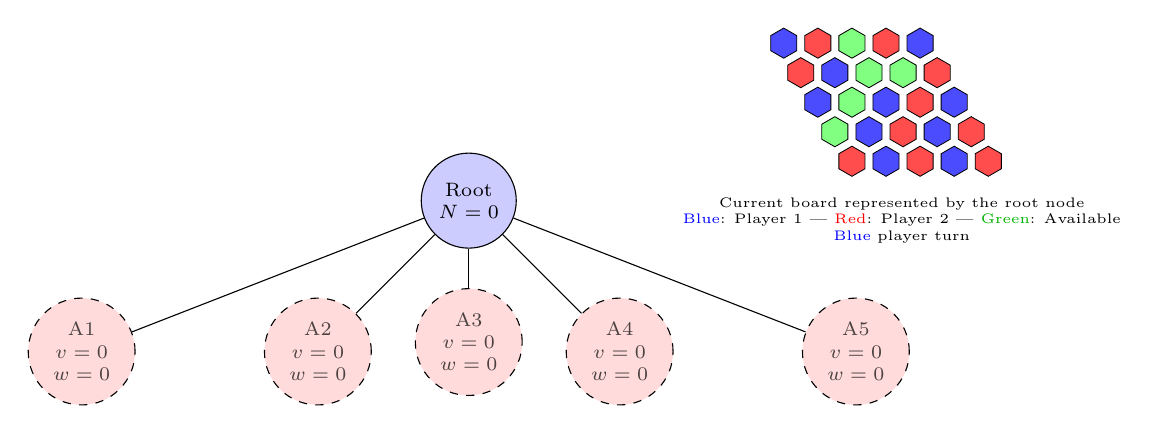
\begin{tikzpicture}[
    node distance=2.35cm,
    treenode/.style={circle, draw, minimum size=1cm, align=center, font=\scriptsize},
    root/.style={treenode, fill=blue!20, font=\scriptsize},
    unvisited/.style={treenode, fill=red!20, fill opacity=0.7, draw, dashed},
    visited/.style={treenode, fill=green!20},
    simulation/.style={rectangle, draw, dashed, fill=yellow!20},
    % Hex board styles
    hexagon/.style={
        regular polygon,
        regular polygon sides=6,
        minimum size=0.33cm,
        draw=black,
        line width=0.3pt,
        rotate=90
    },
    player1/.style={hexagon, fill=blue!70},
    player2/.style={hexagon, fill=red!70},
    available/.style={hexagon, fill=green!50}
]

% Root node
\node[root] (root) {Root\\$N=0$};

% Available moves (unvisited)
\node[unvisited, below left=1cm and 4cm of root] (a1) {A1 \\ $v=0$ \\ $w=0$};
\node[unvisited, below left=1cm and 1cm of root] (a2) {A2 \\ $v=0$ \\ $w=0$};
\node[unvisited, below=0.5cm of root] (a3) {A3 \\ $v=0$ \\ $w=0$};
\node[unvisited, below right=1cm and 1cm of root] (a4) {A4 \\ $v=0$ \\ $w=0$};
\node[unvisited, below right=1cm and 4cm of root] (a5) {A5 \\ $v=0$ \\ $w=0$};

% Edges
\draw (root) -- (a1);
\draw (root) -- (a2);
\draw (root) -- (a3);
\draw (root) -- (a4);
\draw (root) -- (a5);

% Hex board positioning (to the right of root)
\begin{scope}[shift={(4,0.5)}, scale=0.5]
% Define hex grid parameters
\def\hexwidth{0.866}  % sqrt(3)/2
\def\hexheight{0.75}  % 3/4 of the hexagon height

% Draw 5x5 hex board
% Row 1 (top)
\node at (0*\hexwidth, 4*\hexheight) [player1] {};
\node at (1*\hexwidth, 4*\hexheight) [player2] {};
\node at (2*\hexwidth, 4*\hexheight) [available] {};
\node at (3*\hexwidth, 4*\hexheight) [player2] {};
\node at (4*\hexwidth, 4*\hexheight) [player1] {};

% Row 2
\node at (0.5*\hexwidth, 3*\hexheight) [player2] {};
\node at (1.5*\hexwidth, 3*\hexheight) [player1] {};
\node at (2.5*\hexwidth, 3*\hexheight) [available] {};
\node at (3.5*\hexwidth, 3*\hexheight) [available] {};
\node at (4.5*\hexwidth, 3*\hexheight) [player2] {};

% Row 3 (middle)
\node at (1*\hexwidth, 2*\hexheight) [player1] {};
\node at (2*\hexwidth, 2*\hexheight) [available] {};
\node at (3*\hexwidth, 2*\hexheight) [player1] {};
\node at (4*\hexwidth, 2*\hexheight) [player2] {};
\node at (5*\hexwidth, 2*\hexheight) [player1] {};

% Row 4
\node at (1.5*\hexwidth, 1*\hexheight) [available] {};
\node at (2.5*\hexwidth, 1*\hexheight) [player1] {};
\node at (3.5*\hexwidth, 1*\hexheight) [player2] {};
\node at (4.5*\hexwidth, 1*\hexheight) [player1] {};
\node at (5.5*\hexwidth, 1*\hexheight) [player2] {};

% Row 5 (bottom)
\node at (2*\hexwidth, 0*\hexheight) [player2] {};
\node at (3*\hexwidth, 0*\hexheight) [player1] {};
\node at (4*\hexwidth, 0*\hexheight) [player2] {};
\node at (5*\hexwidth, 0*\hexheight) [player1] {};
\node at (6*\hexwidth, 0*\hexheight) [player2] {};

% Small legend
\node at (3, -1.5) [font=\tiny, align=center] {
    Current board represented by the root node \\
    \textcolor{blue}{Blue}: Player 1 | \textcolor{red}{Red}: Player 2 | \textcolor{green!70!black}{Green}: Available \\
    \textcolor{blue}{Blue} player turn
};
\end{scope}

\end{tikzpicture}
\end{center}

\subsubsection*{Iteration 1: First Expansion}

All nodes have UCB1 = $\infty$ (division by zero).
Select any of the possible move. Let's say child A1.
Since A1 is selected the tree is expanded adding a
branch to the tree. Then a simulation is performed
considering that the board is in state represented by
the node A1. During the simulation phase all moves are
performed randomly. It is then the turn of player 2 to
choose a position on the board among the 4 remaining ones.
Suppose that it is the position represented by B2 that was
randomly selected.
If the game did not end then it is the turn again to
player 1 to select a position among the 3 remaining ones.
Suppose it is C2 that is selected.
Then, let's say that with this last move, player 1 won.
The simulation ends and the backpropagation is going to
take place.

\begin{center}
\begin{forest}
    for tree={align=center, font=\scriptsize,s sep=1cm,
    l sep=1.5cm,edge={-Stealth, thin, draw=black!70},circle,
    draw=black!70, dashed, minimum size=1.5cm, inner sep=0pt,},
    root/.style={fill=blue!20, solid, edge={solid, draw=black}},
    unvisited/.style={fill=red!20, fill opacity=0.7, draw, dashed},
    selected/.style={fill=red!20, solid, draw=red,
    line width=0.8pt, edge={-Stealth, thick, red, solid},
    edge label={node[midway, above, font=\small, text=red, sloped]
    {Selected}},
    },
    sim_path/.style={fill=yellow!40, solid, draw=black,
    line width=0.9pt, edge={-Stealth, thick, black, solid}},
    simulation_node/.style={draw, dashed, fill=yellow!20,
    align=center, minimum size=1.5cm, inner sep=2pt,
    s sep=0.1cm, edge={dashed, draw=black!70},
    for children={l sep=0.8cm}},
    where level=0{root}{},
    [{Root \\ $N=0$}, root
        [{A1 \\ $v=0$ \\ $w=0$}, name=A1, selected
            [B1, name=B1, simulation_node],
            [B2, name=B2, sim_path,
                [C1, name=C1, simulation_node],[C2, name=C2,sim_path],
                [C3, name=C3, simulation_node]]
            [B3, name=B3, simulation_node],
            [B4, name=B4, simulation_node]]
        [{A2 \\ $v=0$ \\ $w=0$}, unvisited]
        [{A3 \\ $v=0$ \\ $w=0$}, unvisited]
        [{A4 \\ $v=0$ \\ $w=0$}, unvisited]
        [{A5 \\ $v=0$ \\ $w=0$}, unvisited]
    ]
    \node[
      draw=green, 
      thick, 
      rounded corners, 
      inner sep=5pt, 
      % Fit the node using exact coordinates
      fit={
          ($(B1.north west) + (-0.5em, 0.5em)$) % Top-left coordinate
          ($(B4.south east) + (1em, -0.7em)$)  % Bottom-right coordinate
      },
      % Add the text label 'P2' below the node (90 degrees)
      label={[label distance=-20pt]90:{\textcolor{green}{
        \textbf{P2}}}},
    ] (P2_nodes) {};
    \node[
      draw=brown, 
      thick, 
      rounded corners, 
      inner sep=5pt, 
      % Fit the node using exact coordinates
      fit={
          ($(C1.north west) + (-0.5em, 0.5em)$) % Top-left coordinate
          ($(C3.south east) + (1em, -0.2em)$)  % Bottom-right coordinate
      },
      % Add the text label 'P2' below the node (90 degrees)
      label={[label distance=-45pt]20:{\textcolor{brown}{
        \textbf{P1}}}},
    ] (P1_nodes) {};
    \node[
      draw=blue, 
      thick, 
      rounded corners, 
      fill=blue!10,
      fill opacity=0.3, 
      inner sep=5pt, 
      % Fit the node
      fit={
          ($(B1.north west) + (-1.5em, 2.5em)$) % Top-left coordinate
          ($(C3.south east) + (8em, -2.em)$)  % Bottom-right coordinate
      },
      % Add the text label 'Simulation' above the node (90 degrees)
      label={[label distance=-21pt]45:{\textcolor{blue}{
        \textbf{Simulation}}}},
      label={[label distance=-180pt]91:{\textcolor{black}{
        Simulation Result: \textcolor{blue}{P1 Wins}}}}
    ] (SimulationBox) {};
\end{forest}

\end{center}

\textbf{Backpropagation}: P1 wins $\Rightarrow$ A1: $v=1$, $w=1$,
Root: $N=1$

\textbf{Explanation:} 
\begin{itemize}
    \item $A_1$ gets $w=1$ because it's a Player 1 move and 
    Player 1 won
    \item $A_1$ gets $v=1$ for being visited
    \item Root's $N$ increases to count this iteration
\end{itemize}
\begin{center}
\begin{forest}
    for tree={align=center, font=\scriptsize,s sep=1cm,
    l sep=1.5cm,edge={-Stealth, thin, draw=black!70},circle,
    draw=black!70, dashed, minimum size=1.5cm, inner sep=0pt,},
    root/.style={fill=blue!20, solid, edge={solid, draw=black}},
    unvisited/.style={fill=red!20, fill opacity=0.7, draw, dashed},
    visited/.style={fill=green!20, solid, draw=green,
    line width=0.8pt, edge={-Stealth, thick, black, solid},
    },
    [{Root \\ $N=1$}, root
        [{A1 \\ $v=1$ \\ $w=1$}, name=A1, visited]
        [{A2 \\ $v=0$ \\ $w=0$}, unvisited]
        [{A3 \\ $v=0$ \\ $w=0$}, unvisited]
        [{A4 \\ $v=0$ \\ $w=0$}, unvisited]
        [{A5 \\ $v=0$ \\ $w=0$}, unvisited]
    ]
\end{forest}
\end{center}
%
\vspace{0.5cm}
\noindent
From now on, I will not draw the full simulation path
but just the result of the simulation.

\subsubsection*{Iteration 2: Second Expansion}

Unvisited nodes still have UCB1 = $\infty$. Randomly select A2
among the unvisited child A2, A3, A4 and A5.

\begin{center}
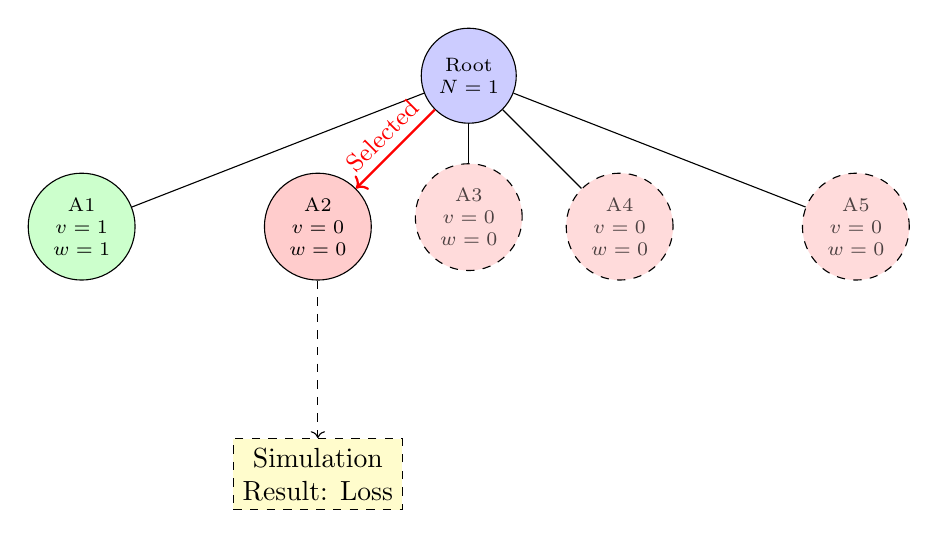
\begin{tikzpicture}[
    node distance=2.35cm,
    treenode/.style={circle, draw, minimum size=1cm, align=center, font=\scriptsize},
    root/.style={treenode, fill=blue!20, font=\scriptsize},
    unvisited/.style={treenode, fill=red!20, fill opacity=0.7, draw, dashed},
    selected/.style={treenode, fill=red!20},
    visited/.style={treenode, fill=green!20},
    simulation/.style={rectangle, draw, dashed, fill=yellow!20, align=center}
]

% Root node
\node[root] (root) {Root \\ $N=1$};

% Previous visited node
\node[visited, below left=1cm and 4cm of root] (a1) {A1 \\ $v=1$ \\ $w=1$};

% A2 is being expanded
\node[selected, below left=1cm and 1cm of root] (a2) {A2 \\ $v=0$ \\ $w=0$};
\node[unvisited, below=0.5cm of root] (a3) {A3 \\ $v=0$ \\ $w=0$};
\node[unvisited, below right=1cm and 1cm of root] (a4) {A4 \\ $v=0$ \\ $w=0$};
\node[unvisited, below right=1cm and 4cm of root] (a5) {A5 \\ $v=0$ \\ $w=0$};

% Simulation cluster
\node[simulation, below=2cm of a2] (sim2) {Simulation \\ Result: Loss};

% Edges and annotations
\draw (root) -- (a1);
\draw[->, thick, red] (root) -- node[above, sloped, font=\small] {Selected} (a2);
\draw (root) -- (a3);
\draw (root) -- (a4);
\draw (root) -- (a5);
\draw[dashed, ->] (a2) -- (sim2);

\end{tikzpicture}
\end{center}

\textbf{Backpropagation}: P1 loses $\Rightarrow$ A2: $v=1$, $w=0$,
Root: $N=2$

\subsubsection*{Iteration 3: Third Expansion}

Select A3 (among the remaining unvisited node A3, A4, A5).

\begin{center}
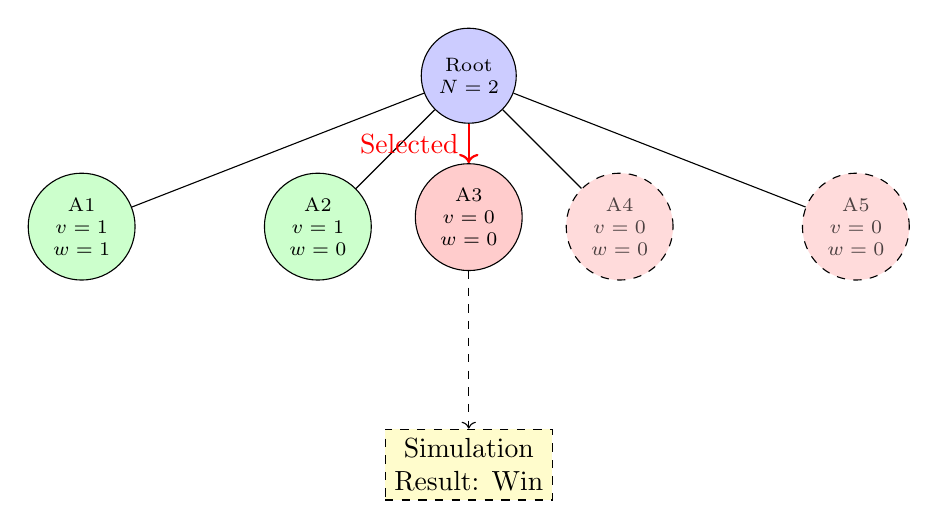
\begin{tikzpicture}[
    node distance=2.35cm,
    treenode/.style={circle, draw, minimum size=1cm, align=center, font=\scriptsize},
    root/.style={treenode, fill=blue!20, font=\scriptsize},
    selected/.style={treenode, fill=red!20},
    unvisited/.style={treenode, fill=red!20, fill opacity=0.7, draw, dashed},
    visited/.style={treenode, fill=green!20},
    simulation/.style={rectangle, draw, dashed, fill=yellow!20, align=center}
]

% Root node
\node[root] (root) {Root \\ $N=2$};

% Previous visited nodes
\node[visited, below left=1cm and 4cm of root] (a1) {A1 \\ $v=1$ \\ $w=1$};
\node[visited, below left=1cm and 1cm of root] (a2) {A2 \\ $v=1$ \\ $w=0$};

% A3 is being expanded
\node[selected, below=0.5cm of root] (a3) {A3 \\ $v=0$ \\ $w=0$};
\node[unvisited, below right=1cm and 1cm of root] (a4) {A4 \\ $v=0$ \\ $w=0$};
\node[unvisited, below right=1cm and 4cm of root] (a5) {A5 \\ $v=0$ \\ $w=0$};

% Simulation cluster
\node[simulation, below=2cm of a3] (sim3) {Simulation \\ Result: Win};

% Edges and annotations
\draw (root) -- (a1);
\draw (root) -- (a2);
\draw[->, thick, red] (root) -- node[left] {Selected} (a3);
\draw (root) -- (a4);
\draw (root) -- (a5);
\draw[dashed, ->] (a3) -- (sim3);

\end{tikzpicture}
\end{center}

\textbf{Backpropagation}: P1 wins $\Rightarrow$ A3: $v=1$, $w=1$,
Root: $N=3$

\subsubsection*{Iteration 4: Fourth Expansion}

Select A4 (among the remaining unvisited node A4 and A5).

\begin{center}
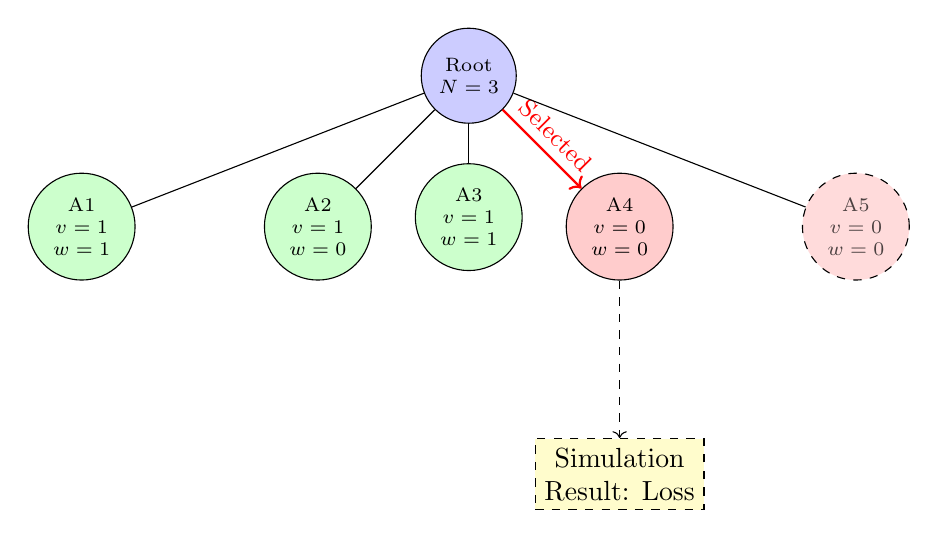
\begin{tikzpicture}[
    node distance=2.35cm,
    treenode/.style={circle, draw, minimum size=1cm, align=center, font=\scriptsize},
    root/.style={treenode, fill=blue!20, font=\scriptsize},
    unvisited/.style={treenode, fill=red!20, fill opacity=0.7, draw, dashed},
    visited/.style={treenode, fill=green!20},
    selected/.style={treenode, fill=red!20},
    simulation/.style={rectangle, draw, dashed, fill=yellow!20, align=center}
]

% Root node
\node[root] (root) {Root \\ $N=3$};

% Previous visited nodes
\node[visited, below left=1cm and 4cm of root] (a1) {A1 \\ $v=1$ \\ $w=1$};
\node[visited, below left=1cm and 1cm of root] (a2) {A2 \\ $v=1$ \\ $w=0$};
\node[visited, below=0.5cm of root] (a3) {A3 \\ $v=1$ \\ $w=1$};

% A4 is being expanded
\node[selected, below right=1cm and 1cm of root] (a4) {A4 \\ $v=0$ \\ $w=0$};
\node[unvisited, below right=1cm and 4cm of root] (a5) {A5 \\ $v=0$ \\ $w=0$};

% Simulation cluster
\node[simulation, below=2cm of a4] (sim4) {Simulation \\ Result: Loss};

% Edges and annotations
\draw (root) -- (a1);
\draw (root) -- (a2);
\draw (root) -- (a3);
\draw[->, thick, red] (root) -- node[above, sloped, font=\small] {Selected} (a4);
\draw (root) -- (a5);
\draw[dashed, ->] (a4) -- (sim4);

\end{tikzpicture}
\end{center}

\textbf{Backpropagation}: P1 loses $\Rightarrow$ A4: $v=1$, $w=0$,
Root: $N=4$

\subsubsection*{Iteration 5: Final Initial Expansion}

Select A5 (last unvisited node).

\begin{center}
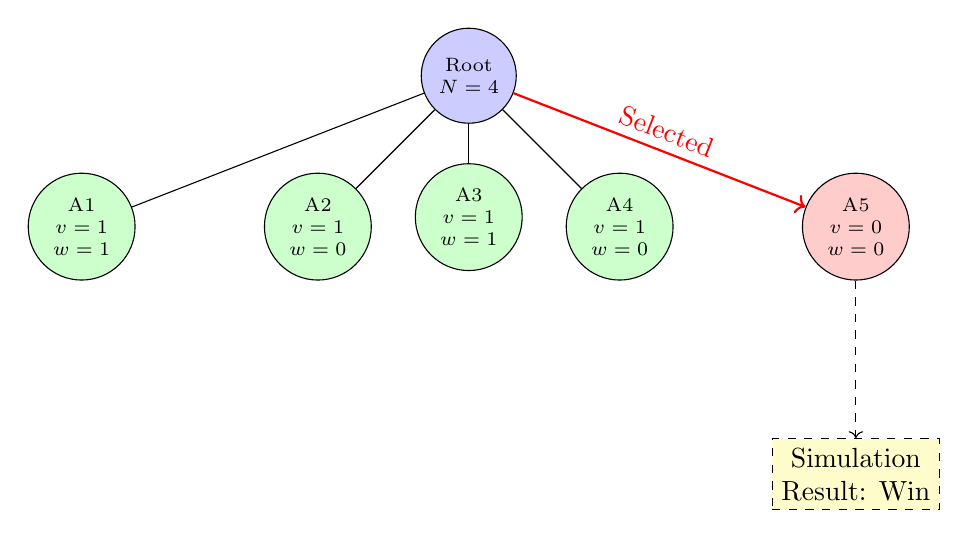
\begin{tikzpicture}[
    node distance=2.35cm,
    treenode/.style={circle, draw, minimum size=1cm, align=center, font=\scriptsize},
    root/.style={treenode, fill=blue!20, font=\scriptsize},
    unvisited/.style={treenode, fill=red!20, fill opacity=0.7, draw, dashed},
    visited/.style={treenode, fill=green!20},
    selected/.style={treenode, fill=red!20},
    simulation/.style={rectangle, draw, dashed, fill=yellow!20, align=center}
]

% Root node
\node[root] (root) {Root \\ $N=4$};

% All nodes now visited
\node[visited, below left=1cm and 4cm of root] (a1) {A1 \\ $v=1$ \\ $w=1$};
\node[visited, below left=1cm and 1cm of root] (a2) {A2 \\ $v=1$ \\ $w=0$};
\node[visited, below=0.5cm of root] (a3) {A3 \\ $v=1$ \\ $w=1$};
\node[visited, below right=1cm and 1cm of root] (a4) {A4 \\ $v=1$ \\ $w=0$};

% A5 is being expanded (last one)
\node[selected, below right=1cm and 4cm of root] (a5) {A5 \\ $v=0$ \\ $w=0$};

% Simulation cluster
\node[simulation, below=2cm of a5] (sim5) {Simulation \\ Result: Win};

% Edges and annotations
\draw (root) -- (a1);
\draw (root) -- (a2);
\draw (root) -- (a3);
\draw (root) -- (a4);
\draw[->, thick, red] (root) -- node[above, sloped] {Selected} (a5);
\draw[dashed, ->] (a5) -- (sim5);

\end{tikzpicture}
\end{center}

\textbf{Backpropagation}: P1 wins $\Rightarrow$ A5: $v=1$, $w=1$,
Root: $N=5$

\begin{center}
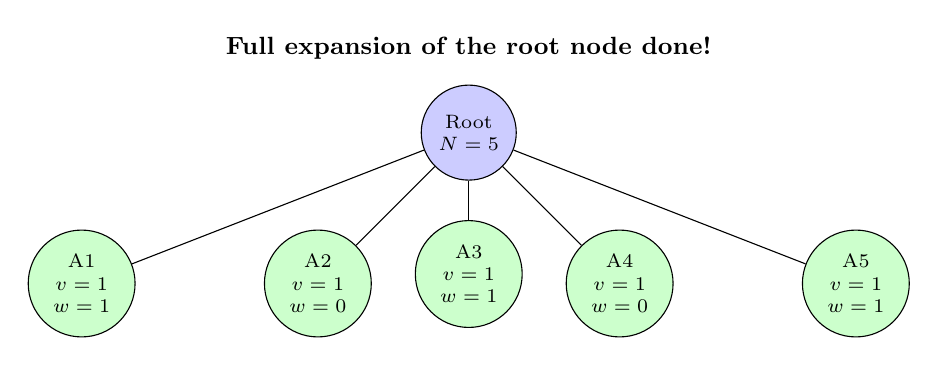
\begin{tikzpicture}[
    node distance=2.35cm,
    treenode/.style={circle, draw, minimum size=1cm, align=center, font=\scriptsize},
    root/.style={treenode, fill=blue!20, font=\scriptsize},
    unvisited/.style={treenode, fill=red!20, fill opacity=0.7, draw, dashed},
    visited/.style={treenode, fill=green!20},
    selected/.style={treenode, fill=red!20},
    simulation/.style={rectangle, draw, dashed, fill=yellow!20, align=center}
]

% Root node
\node[root] (root) {Root \\ $N=5$};

% All nodes now visited
\node[visited, below left=1cm and 4cm of root] (a1) {A1 \\ $v=1$ \\ $w=1$};
\node[visited, below left=1cm and 1cm of root] (a2) {A2 \\ $v=1$ \\ $w=0$};
\node[visited, below=0.5cm of root] (a3) {A3 \\ $v=1$ \\ $w=1$};
\node[visited, below right=1cm and 1cm of root] (a4) {A4 \\ $v=1$ \\ $w=0$};
\node[visited, below right=1cm and 4cm of root] (a5) {A5 \\ $v=1$ \\ $w=1$};

% Edges and annotations
\draw (root) -- (a1);
\draw (root) -- (a2);
\draw (root) -- (a3);
\draw (root) -- (a4);
\draw (root) -- (a5);

\node[above=0.2cm of root] {\small\textbf{Full expansion of the root node done!}};

\end{tikzpicture}
\end{center}

\subsubsection*{Iteration 6: First (real) UCB1 Selection}

Now all nodes have been visited once (the root node is fully expanded
and it is not a terminal node). Calculate UCB1 ($c = \sqrt{2}$):

\begin{align*}
\text{UCB1}(A1) &= \frac{1}{1} + \sqrt{2} \sqrt{\frac{\ln 5}{1}} = 1 + 1.79 = 2.79 \\
\text{UCB1}(A2) &= \frac{0}{1} + \sqrt{2} \sqrt{\frac{\ln 5}{1}} = 0 + 1.79 = 1.79 \\
\text{UCB1}(A3) &= \frac{1}{1} + \sqrt{2} \sqrt{\frac{\ln 5}{1}} = 1 + 1.79 = 2.79 \\
\text{UCB1}(A4) &= \frac{0}{1} + \sqrt{2} \sqrt{\frac{\ln 5}{1}} = 0 + 1.79 = 1.79 \\
\text{UCB1}(A5) &= \frac{1}{1} + \sqrt{2} \sqrt{\frac{\ln 5}{1}} = 1 + 1.79 = 2.79
\end{align*}

Tie between A1, A3, A5. Randomly select A1.

\begin{center}
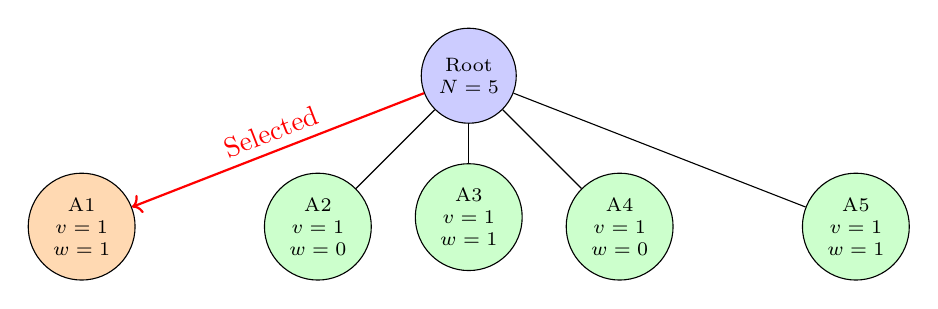
\begin{tikzpicture}[
    node distance=2.35cm,
    treenode/.style={circle, draw, minimum size=1cm, align=center, font=\scriptsize},
    root/.style={treenode, fill=blue!20, font=\scriptsize},
    visited/.style={treenode, fill=green!20},
    selected/.style={treenode, fill=orange!30},
    simulation/.style={rectangle, draw, dashed, fill=yellow!20, align=center}
]

% Root node
\node[root] (root) {Root \\ $N=5$};

% All nodes visited
\node[selected, below left=1cm and 4cm of root] (a1) {A1 \\ $v=1$ \\ $w=1$};
\node[visited, below left=1cm and 1cm of root] (a2) {A2 \\ $v=1$ \\ $w=0$};
\node[visited, below=0.5cm of root] (a3) {A3 \\ $v=1$ \\ $w=1$};
\node[visited, below right=1cm and 1cm of root] (a4) {A4 \\ $v=1$ \\ $w=0$};
\node[visited, below right=1cm and 4cm of root] (a5) {A5 \\ $v=1$ \\ $w=1$};

% Edges and annotations
\draw[->, thick, red] (root) -- node[above, sloped] {Selected} (a1);
\draw (root) -- (a2);
\draw (root) -- (a3);
\draw (root) -- (a4);
\draw (root) -- (a5);

\end{tikzpicture}
\end{center}

Then expand the selected child node A1.
So, for the position that could occupy player 2, there is the choice
between B1, B2, B3 and B4. Let's say B4 is selected (for example
it is popped from the end of the list of available moves).

\begin{figure}[h]
\begin{center}
\begin{forest}
    for tree={align=center, font=\scriptsize,s sep=1cm,
    l sep=1.5cm,edge={-Stealth, thin, draw=black!70},circle,
    draw=black!70, dashed, minimum size=1.5cm, inner sep=0pt,},
    root/.style={fill=blue!20, solid, edge={solid, draw=black}},
    unvisited/.style={fill=red!20, fill opacity=0.7, draw, dashed},
    visited/.style={fill=green!20, solid, draw=green,
    line width=0.8pt, edge={-Stealth, thick, black, solid}},
    selected/.style={fill=red!20, solid, draw=red,
    line width=0.8pt, edge={-Stealth, thick, red, solid},
    edge label={node[midway, above, font=\small, text=red, sloped]
    {Selected}},
    },
    expansion_candidate/.style={dashed, draw=black,
    line width=0.9pt, edge={-Stealth, thick, black, dashed}},
    simulation_node/.style={draw, dashed, fill=yellow!20,
    align=center, minimum size=1.5cm, inner sep=2pt,
    s sep=0.1cm, edge={dashed, draw=black!70},
    for children={l sep=0.8cm}},
    where level=0{root}{},
    [{Root \\ $N=5$}, root
        [{A1 \\ $v=1$ \\ $w=1$}, name=A1, selected
            [B1, name=B1, expansion_candidate],
            [B2, name=B2, expansion_candidate],
            [B3, name=B3, expansion_candidate],
            [B4, name=B4, selected]]
        [{A2 \\ $v=1$ \\ $w=0$}, visited]
        [{A3 \\ $v=1$ \\ $w=1$}, visited]
        [{A4 \\ $v=1$ \\ $w=0$}, visited]
        [{A5 \\ $v=1$ \\ $w=1$}, visited]
    ];
    \node[
      draw=gray, 
      dashed, 
      rounded corners, 
      inner sep=5pt, 
      % Fit the node using exact coordinates
      fit={
          ($(A1.north west) + (-4.5em, -3.5em)$) % Top-left coordinate
          ($(A5.south east) + (14em, -5em)$)  % Bottom-right coordinate
      },
      % Add the text label 'P2' below the node (90 degrees)
      label={[label distance=-50pt]180:{\textcolor{gray}{
        \textbf{P1}}}},
    ] (P1_nodes) {};
    \node[
      draw=gray, 
      dashed, 
      rounded corners, 
      inner sep=5pt, 
      % Fit the node using exact coordinates
      fit={
          ($(B1.north west) + (-0.5em, 0.5em)$) % Top-left coordinate
          ($(B4.south east) + (3em, -0.7em)$)  % Bottom-right coordinate
      },
      % Add the text label 'P2' below the node (90 degrees)
      label={[label distance=-35pt]2:{\textcolor{gray}{
        \textbf{P2}}}},
    ] (P2_nodes) {};
\end{forest}
%
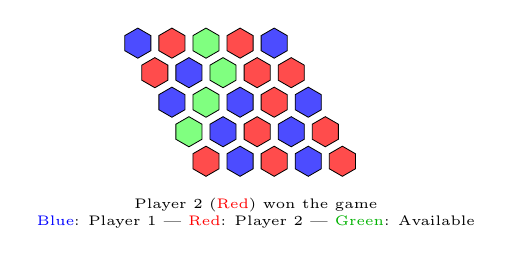
\begin{tikzpicture}[
    node distance=2.35cm,
    % Hex board styles
    hexagon/.style={
        regular polygon,
        regular polygon sides=6,
        minimum size=0.33cm,
        draw=black,
        line width=0.3pt,
        rotate=90
    },
    player1/.style={hexagon, fill=blue!70},
    player2/.style={hexagon, fill=red!70},
    available/.style={hexagon, fill=green!50}
]

% Hex board positioning (to the right of root)
\begin{scope}[shift={(4,0.5)}, scale=0.5]
% Define hex grid parameters
\def\hexwidth{0.866}  % sqrt(3)/2
\def\hexheight{0.75}  % 3/4 of the hexagon height

% Draw 5x5 hex board
% Row 1 (top)
\node at (0*\hexwidth, 4*\hexheight) [player1] {};
\node at (1*\hexwidth, 4*\hexheight) [player2] {};
\node at (2*\hexwidth, 4*\hexheight) [available] {};
\node at (3*\hexwidth, 4*\hexheight) [player2] {};
\node at (4*\hexwidth, 4*\hexheight) [player1] {};

% Row 2
\node at (0.5*\hexwidth, 3*\hexheight) [player2] {};
\node at (1.5*\hexwidth, 3*\hexheight) [player1] {};
\node at (2.5*\hexwidth, 3*\hexheight) [available] {};
\node at (3.5*\hexwidth, 3*\hexheight) [player2] {};
\node at (4.5*\hexwidth, 3*\hexheight) [player2] {};

% Row 3 (middle)
\node at (1*\hexwidth, 2*\hexheight) [player1] {};
\node at (2*\hexwidth, 2*\hexheight) [available] {};
\node at (3*\hexwidth, 2*\hexheight) [player1] {};
\node at (4*\hexwidth, 2*\hexheight) [player2] {};
\node at (5*\hexwidth, 2*\hexheight) [player1] {};

% Row 4
\node at (1.5*\hexwidth, 1*\hexheight) [available] {};
\node at (2.5*\hexwidth, 1*\hexheight) [player1] {};
\node at (3.5*\hexwidth, 1*\hexheight) [player2] {};
\node at (4.5*\hexwidth, 1*\hexheight) [player1] {};
\node at (5.5*\hexwidth, 1*\hexheight) [player2] {};

% Row 5 (bottom)
\node at (2*\hexwidth, 0*\hexheight) [player2] {};
\node at (3*\hexwidth, 0*\hexheight) [player1] {};
\node at (4*\hexwidth, 0*\hexheight) [player2] {};
\node at (5*\hexwidth, 0*\hexheight) [player1] {};
\node at (6*\hexwidth, 0*\hexheight) [player2] {};

% Small legend
\node at (3, -1.5) [font=\tiny, align=center] {
    Player 2 (\textcolor{red}{Red}) won the game \\
    \textcolor{blue}{Blue}: Player 1 | \textcolor{red}{Red}: Player 2 | \textcolor{green!70!black}{Green}: Available \\
};
\end{scope}
\end{tikzpicture}

\end{center}
  %\caption{TikZ picture next to a Forest tree.}
\end{figure}
%
Has it happened, by selecting the move (represented by) B2, player 2
wins the game (hence player 1 lost it).\\
The tree is updated accordingly (backpropagation):
\begin{itemize}
    \item B4: $v = 1$, $w = 1$
    \item A1: $v = v + 1 = 2$, $w = w + 0 = 1$
    \item N: $N = N + 1 = 6$
\end{itemize}

\textbf{Key observation:} $B_4$ gets $w=1$ because it's a 
Player 2 move and Player 2 won. $A_1$ doesn't increase its 
win count because Player 1 lost. This is the minimax 
perspective in action!
\begin{center}
\begin{forest}
    for tree={align=center, font=\scriptsize,s sep=1cm,
    l sep=1.5cm,edge={-Stealth, thin, draw=black!70},circle,
    draw=black!70, dashed, minimum size=1.5cm, inner sep=0pt,},
    root/.style={fill=blue!20, solid, edge={solid, draw=black}},
    unvisited/.style={fill=red!20, fill opacity=0.7, draw, dashed},
    visited/.style={fill=green!20, solid, draw=green,
    line width=0.8pt, edge={-Stealth, thick, black, solid}},
    selected/.style={fill=red!20, solid, draw=red,
    line width=0.8pt, edge={-Stealth, thick, red, solid},
    edge label={node[midway, above, font=\small, text=red, sloped]
    {Selected}}
    },
    expansion_candidate/.style={dashed, draw=black,
    line width=0.9pt, edge={-Stealth, thick, black, dashed}},
    simulation_node/.style={draw, dashed, fill=yellow!20,
    align=center, minimum size=1.5cm, inner sep=2pt,
    s sep=0.1cm, edge={dashed, draw=black!70},
    for children={l sep=0.8cm}},
    where level=0{root}{},
    [{Root \\ $N=6$}, root
            [A1 {\\ $v=\mathbf{2}$ \\ $w=\mathbf{1}$}, name=A1, visited,
            [{B4 \\ $v=1$ \\ $w=\mathbf{1}$}, name=B4, visited]]
        [{A2 \\ $v=1$ \\ $w=0$}, visited]
        [{A3 \\ $v=1$ \\ $w=1$}, visited]
        [{A4 \\ $v=1$ \\ $w=0$}, visited]
        [{A5 \\ $v=1$ \\ $w=1$}, visited]
    ];
    \node[
      draw=gray, 
      dashed, 
      rounded corners, 
      inner sep=5pt, 
      % Fit the node using exact coordinates
      fit={
          ($(A1.north west) + (-4.5em, -3.5em)$) % Top-left coordinate
          ($(A5.south east) + (14em, -5em)$)  % Bottom-right coordinate
      },
      % Add the text label 'P2' below the node (90 degrees)
      label={[label distance=-50pt]180:{\textcolor{gray}{
        \textbf{P1}}}},
    ] (P1_nodes) {};
    \node[
      draw=gray, 
      dashed, 
      rounded corners, 
      inner sep=5pt, 
      % Fit the node using exact coordinates
      fit={
          ($(B4.north west) + (-0.5em, 0.5em)$) % Top-left coordinate
          ($(B4.south east) + (3em, -0.7em)$)  % Bottom-right coordinate
      },
      % Add the text label 'P2' below the node (90 degrees)
      label={[label distance=-35pt]2:{\textcolor{gray}{
        \textbf{P2}}}},
    ] (P2_nodes) {};
\end{forest}
\end{center}

Unless the time credit or iteration credit expired, the process
goes on.\\
So, we are back to selection step, starting from the root node.\\
Calculate UCB1 ($c = \sqrt{2}$):

\begin{align*}
\text{UCB1}(A1) &= \frac{1}{2} + \sqrt{2} \sqrt{\frac{\ln 6}{2}} = 0.5 + 1.89 = 2.39 \\
\text{UCB1}(A2) &= \frac{0}{1} + \sqrt{2} \sqrt{\frac{\ln 6}{1}} = 0 + 1.89 = 1.89 \\
\text{UCB1}(A3) &= \frac{1}{1} + \sqrt{2} \sqrt{\frac{\ln 6}{1}} = 1 + 1.89 = 2.89 \\
\text{UCB1}(A4) &= \frac{0}{1} + \sqrt{2} \sqrt{\frac{\ln 6}{1}} = 0 + 1.89 = 1.89 \\
\text{UCB1}(A5) &= \frac{1}{1} + \sqrt{2} \sqrt{\frac{\ln 6}{1}} = 1 + 1.89 = 2.89
\end{align*}

Tie between A3, A5. Randomly select A3.\\
Then expand the selected child node A3.
So, for the position that could occupy player 2, there is now the choice
between D1, D2, D3 and D4.\\
Let's say D4 is selected.\\
The simulation then take place. There are 3 moves available for
player 1, represented by E1, E2 and E3.
Suppose E2 is chosen.
There remains 2 moves possible for player 2, represented by F1 and F2.
Let's say F1 is selected which terminate the game with the
player 2 losing (i.e. player 1 wins).

\begin{center}
\begin{forest}
    for tree={align=center, font=\scriptsize,s sep=1cm,
    l sep=1.5cm,edge={-Stealth, thin, draw=black!70},circle,
    draw=black!70, dashed, minimum size=1.5cm, inner sep=0pt,},
    root/.style={fill=blue!20, solid, edge={solid, draw=black}},
    unvisited/.style={fill=red!20, fill opacity=0.7, draw, dashed},
    visited/.style={fill=green!20, solid, draw=green,
    line width=0.8pt, edge={-Stealth, thick, black, solid}},
    selected/.style={fill=red!20, solid, draw=red,
    line width=0.8pt, edge={-Stealth, thick, red, solid},
    edge label={node[midway, above, font=\small, text=red, sloped]
    {Selected}},
    },
    expansion_candidate/.style={dashed, draw=black,
    line width=0.9pt, edge={-Stealth, thick, black, dashed}},
    simulation_node/.style={draw, dashed, fill=yellow!20,
    align=center, minimum size=1.5cm, inner sep=2pt,
    s sep=0.1cm, edge={dashed, draw=black!70},
    for children={l sep=0.8cm}},
    sim_path/.style={fill=yellow!40, solid, draw=black,
    line width=0.9pt, edge={-Stealth, thick, black, solid}},
    where level=0{root}{},
    [{Root \\ $N=6$}, root
        [{A1 \\ $v=2$ \\ $w=1$}, name=A1, visited,
            [{B4 \\ $v=1$ \\ $w=\mathbf{1}$}, name=B4, visited]]
        [{A2 \\ $v=1$ \\ $w=0$}, name=A2,visited]
        [{A3 \\ $v=1$ \\ $w=1$}, name=A3,selected,
            [D1, name=D1, expansion_candidate],
            [D2, name=D2, expansion_candidate],
            [D3, name=D3, expansion_candidate],
            [{D4 \\ $v=0$ \\ $w=0$}, name=D4, selected
                [E1, name=E1, simulation_node],
                [E2, name=E2, sim_path,
                    [F1, name=F1, sim_path],
                    [F2, name=F2, simulation_node]]
                [E3, name=E3, simulation_node]]]
        [{A4 \\ $v=1$ \\ $w=0$}, visited]
        [{A5 \\ $v=1$ \\ $w=1$}, visited]
    ];
    \node[
      draw=gray, 
      dashed, 
      rounded corners, 
      inner sep=5pt, 
      % Fit the node using exact coordinates
      fit={
          ($(A1.north west) + (-2.5em, -2.9em)$) % Top-left coordinate
          ($(A5.south east) + (16em, -6em)$)  % Bottom-right coordinate
      },
      % Add the text label 'P2' below the node (90 degrees)
      label={[label distance=-30pt]95:{\textcolor{gray}{
        \textbf{P1}}}},
    ] (P1_1_nodes) {};
    \node[
      draw=gray, 
      dashed, 
      rounded corners, 
      inner sep=5pt, 
      % Fit the node using exact coordinates
      fit={
          ($(B4.north west) + (-0.5em, 0.5em)$) % Top-left coordinate
          ($(B4.south east) + (26em, -0.9em)$)  % Bottom-right coordinate
      },
      % Add the text label 'P2' below the node (90 degrees)
      label={[label distance=-35pt]5:{\textcolor{gray}{
        \textbf{P2}}}},
    ] (P2_1_nodes) {};
    \node[
      draw=gray, 
      dashed, 
      rounded corners, 
      inner sep=5pt, 
      % Fit the node using exact coordinates
      fit={
          ($(E1.north west) + (-1.0em, 1.0em)$) % Top-left coordinate
          ($(E3.south east) + (0.5em, -1em)$)  % Bottom-right coordinate
      },
      % Add the text label 'P2' below the node (90 degrees)
      label={[label distance=-41pt]31:{\textcolor{gray}{
        \textbf{P1}}}},
    ] (P1_2_nodes) {};
    \node[
      draw=gray, 
      dashed, 
      rounded corners, 
      inner sep=5pt, 
      % Fit the node using exact coordinates
      fit={
          ($(F1.north west) + (-0.5em, 0.5em)$) % Top-left coordinate
          ($(F2.south east) + (3em, -0.7em)$)  % Bottom-right coordinate
      },
      % Add the text label 'P2' below the node (90 degrees)
      label={[label distance=-85pt]30:{\textcolor{gray}{
        \textbf{P2}}}},
    ] (P2_2_nodes) {};
    \node[
      draw=blue, 
      thick, 
      rounded corners, 
      fill=blue!10,
      fill opacity=0.3, 
      inner sep=5pt, 
      % Fit the node
      fit={
          ($(E1.north west) + (-1.5em, 2.5em)$) % Top-left coordinate
          ($(F2.south east) + (8em, -2.em)$)  % Bottom-right coordinate
      },
      % Add the text label 'Simulation' above the node (90 degrees)
      label={[label distance=-21pt]65:{\textcolor{blue}{
        \textbf{Simulation}}}},
      label={[label distance=-180pt]91:{\textcolor{black}{
        Simulation Result: \textcolor{blue}{P1 Wins}}}}
    ] (SimulationBox) {};
\end{forest}
\end{center}

Once the simulation is done, the backpropagation is performed.\\
Since player 1 won, we have the updates:
\begin{itemize}
    \item D4: $v = 1$, $w = 0$
    \item A3: $v = v + 1 = 2$, $w = w + 1 = 2$
    \item N: $N = N + 1 = 7$
\end{itemize}

\begin{center}
\begin{forest}
    for tree={align=center, font=\scriptsize,s sep=1cm,
    l sep=1.5cm,edge={-Stealth, thin, draw=black!70},circle,
    draw=black!70, dashed, minimum size=1.5cm, inner sep=0pt,},
    root/.style={fill=blue!20, solid, edge={solid, draw=black}},
    unvisited/.style={fill=red!20, fill opacity=0.7, draw, dashed},
    visited/.style={fill=green!20, solid, draw=green,
    line width=0.8pt, edge={-Stealth, thick, black, solid}},
    selected/.style={fill=red!20, solid, draw=red,
    line width=0.8pt, edge={-Stealth, thick, red, solid},
    edge label={node[midway, above, font=\small, text=red, sloped]
    {Selected}},
    },
    expansion_candidate/.style={dashed, draw=black,
    line width=0.9pt, edge={-Stealth, thick, black, dashed}},
    simulation_node/.style={draw, dashed, fill=yellow!20,
    align=center, minimum size=1.5cm, inner sep=2pt,
    s sep=0.1cm, edge={dashed, draw=black!70},
    for children={l sep=0.8cm}},
    where level=0{root}{},
    [{Root \\ $N=7$}, root
            [A1 {\\ $v=2$ \\ $w=1$}, name=A1, visited,
            [{B4 \\ $v=1$ \\ $w=1$}, name=B4, visited]]
        [{A2 \\ $v=1$ \\ $w=0$}, visited]
        [{A3 \\ $v=2$ \\ $w=\mathbf{2}$}, visited,
            [{D4 \\ $v=1$ \\ $w=\mathbf{0}$}, name=D4, visited]]
        [{A4 \\ $v=1$ \\ $w=0$}, visited]
        [{A5 \\ $v=1$ \\ $w=1$}, visited]
    ];
    \node[
      draw=gray, 
      dashed, 
      rounded corners, 
      inner sep=5pt, 
      % Fit the node using exact coordinates
      fit={
          ($(A1.north west) + (-2.2em, -3.5em)$) % Top-left coordinate
          ($(A5.south east) + (14em, -5em)$)  % Bottom-right coordinate
      },
      % Add the text label 'P1'
      label={[label distance=-20pt]180:{\textcolor{gray}{
        \textbf{P1}}}},
    ] (P1_nodes) {};
    \node[
      draw=gray, 
      dashed, 
      rounded corners, 
      inner sep=5pt, 
      % Fit the node using exact coordinates
      fit={
          ($(B4.north west) + (-0.5em, 0.5em)$) % Top-left coordinate
          ($(B4.south east) + (13em, -0.7em)$)  % Bottom-right coordinate
      },
      % Add the text label 'P2'
      label={[label distance=-35pt]60:{\textcolor{gray}{
        \textbf{P2}}}},
    ] (P2_nodes) {};
\end{forest}
\end{center}
And we are ready to start a new iteration from the root node.

\begin{itemize}
\item $\text{UCB1}(A1) = \frac{1}{2} + \sqrt{2} \sqrt{\frac{\ln 7}{2}} = 0.5 + \sqrt{\ln 7} = 0.5 + 1.39496 = 1.895$ 
\item $\text{UCB1}(A2) = \frac{0}{1} + \sqrt{2} \sqrt{\frac{\ln 7}{1}} = 0 + \sqrt{2\ln 7} = 0 + 1.97299 = 1.973$ 
\item $\text{UCB1}(A3) = \frac{2}{2} + \sqrt{2} \sqrt{\frac{\ln 7}{1}} = 1 + \sqrt{2\ln 7} = 1 + 1.97299 = 2.973$ 
\item $\text{UCB1}(A4) = \frac{0}{1} + \sqrt{2} \sqrt{\frac{\ln 7}{1}} = 0 + \sqrt{2\ln 7} = 0 + 1.97299 = 1.973$
\item $\text{UCB1}(A5) = \frac{1}{1} + \sqrt{2} \sqrt{\frac{\ln 7}{1}} = 1 + \sqrt{2\ln 7} = 1 + 1.97299 = 2.973$
\end{itemize} 

We have 2 winners, A3 and A5.
Let's say A3 is selected, then as it is not a terminal node and
it is not fully expanded, one of its children (D1, D2, or D3) is going
to be selected for the expansion of the tree\footnote{They all have 
$UCB1 = \infty$ so there is no preference.}.

This process continues for many iterations (typically hundreds 
to thousands), gradually building up the tree and improving 
win rate estimates.

\section*{Final Move Selection}

After all iterations are complete, how do we decide which move 
to actually play? There are several common strategies:

\subsection*{Most Visits (Recommended)}

Select the child of the root with the highest visit count:

\[
\text{Best move} = \arg\max_i v_i
\]

This is the most robust strategy because:
\begin{itemize}
    \item Visit counts are more stable than win rates
    \item A highly-visited node has been thoroughly explored
    \item The UCB1 formula naturally directs visits toward 
    promising moves
\end{itemize}

\subsection*{Highest Win Rate}

Select the child with the highest win rate:

\[
\text{Best move} = \arg\max_i \frac{w_i}{v_i}
\]

This can be overly optimistic, especially for less-visited 
nodes. Generally less reliable than the visit-count method.

\subsection*{Robust Child (Max-Robust)}

Select the child that maximizes a lower confidence bound:

\[
\text{Best move} = \arg\max_i \left(\frac{w_i}{v_i} - 
c\sqrt{\frac{\ln N}{v_i}}\right)
\]

This is a pessimistic approach that guards against uncertainty.

\subsection*{Example Final Selection}

From our example after iteration 7, the visit counts are:
\begin{itemize}
    \item $A_1$: $v = 2$, $w = 1$ (win rate: 50\%)
    \item $A_2$: $v = 1$, $w = 0$ (win rate: 0\%)
    \item $A_3$: $v = 2$, $w = 2$ (win rate: 100\%)
    \item $A_4$: $v = 1$, $w = 0$ (win rate: 0\%)
    \item $A_5$: $v = 1$, $w = 1$ (win rate: 100\%)
\end{itemize}

With more iterations, one move would clearly emerge as having 
both high visit count and high win rate. The most-visited node 
strategy would be the standard choice.

\section*{Key Insights and Best Practices}

\subsection*{Why MCTS Works}

\begin{enumerate}
    \item \textbf{No evaluation function needed}: Random 
    playouts provide position estimates without domain knowledge
    \item \textbf{Adaptive exploration}: UCB1 automatically 
    balances exploring new moves and exploiting good ones
    \item \textbf{Asymmetric tree growth}: More computational 
    effort is spent on promising branches
    \item \textbf{Any-time algorithm}: Can be stopped at any 
    point and return the best move found so far
\end{enumerate}

\subsection*{Practical Considerations}

\begin{itemize}
    \item \textbf{Exploration constant}: $c = \sqrt{2}$ is 
    theoretically optimal for the multi-armed bandit problem, 
    but can be tuned for specific games
    \item \textbf{Progressive widening}: For games with large 
    branching factors, consider expanding only a subset of 
    children initially
    \item \textbf{Domain knowledge}: While MCTS works with 
    random playouts, incorporating heuristics in the simulation 
    phase can improve performance
    \item \textbf{Parallelization}: Multiple simulations can 
    run in parallel, though care must be taken with tree updates
\end{itemize}

\subsection*{When to Use MCTS}

MCTS is particularly effective for:
\begin{itemize}
    \item Games with large state spaces where minimax with 
    alpha-beta pruning is impractical
    \item Domains where it's hard to design good evaluation 
    functions
    \item Any-time scenarios where you need to return a 
    reasonable move quickly but can improve given more time
    \item Two-player zero-sum games (though variants exist for 
    other settings)
\end{itemize}

\section*{Conclusion}

Monte Carlo Tree Search elegantly combines three powerful ideas:
\begin{itemize}
    \item \textbf{Minimax structure} for adversarial reasoning
    \item \textbf{Monte Carlo evaluation} for estimating 
    position values
    \item \textbf{UCB1 selection} for balancing exploration 
    and exploitation
\end{itemize}

This combination has proven highly successful in game AI, 
most famously in AlphaGo's victory over human champions in Go. 
The algorithm's simplicity, effectiveness, and ability to work 
without domain-specific evaluation functions make it a powerful 
tool for a wide range of applications.

\end{document}